
\subsubsection{KW50: 13.12.2021 bis 20.12.2021}
\begin{quote}
	\subsubsection*{Arbeit in der Schule}
	Charakter Direktorin erstellt
	Charakterskin und Animationen von Mixamo.com geholt
	Animation: einfaches ide zum stehen
	
	
	Meine nächste Aufgabe:
	Dialog mit Lehrer programmierten: Wenn Schüler in in der Nähe vom Lehrer oder Direktorin ist, startet eine Konversation. 
	Beim Dialog stellt der Lehrer nach einem kurzen Gespräch fragen an den Schüler.
	Schüler kann mit Buttons auf die Fragen antworten.
	Wenn auf Fragen falsch beantwortet wird, wird sein leben weniger.
	\subsubsection*{Arbeit außerhalb der Schule}
	
	create Empty DialogueSystem: hier werden unsere Dialog GUIs sein, die mit dem Script DialogueSystem verwaltet werden
	1. GUI DialogueUI: Hier werden die Gespräche im Textbox angezeigt
	2. DialogueUI Question Buttons: Dieses GUI wird angezeigt, wenn der Lehrer, dem Schüler eine Frage stellt
	
	
	\begin{figure}
		\centering
		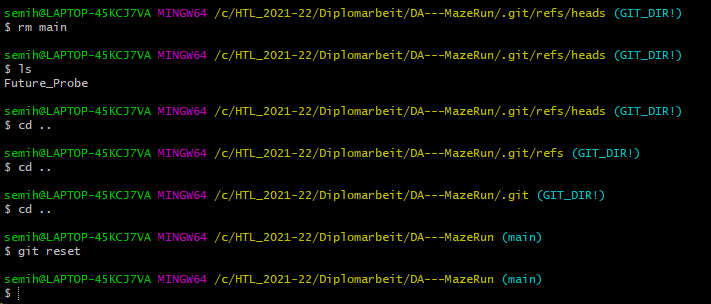
\includegraphics[width=0.7\linewidth]{img/SemihSoenmez_IMG/screenshot02}
		\caption{}
		\label{fig:screenshot02}
	\end{figure}
	
	In meiner Git Repository konnte ich den Main Branch nicth finden. Anschließend habe ich folgende Befehle verwendet um das Problem zu lösen.
	


\end{quote}
